\documentclass[12pt]{../notes}

% Command for Questions
%\question{}

% Command for Notes
% \note{}

% Code to create a minipage where you can type in class notes. 
%%\begin{minipage}[l][2cm][c]{\textwidth}
%\begin{comment}

%\end{comment}
%%\end{minipage}


% Begin Document
%==============================================================================
\begin{document}
% Include the Title of the Handout
\ntitle{6.1: Introduction to Time Series}

\section{Why Time Series?}
Recall our basic multiple linear regression model:
\begin{eqnarray}
  Y_t & = & \beta_0 + \beta_1 X_{t,1} + \ldots + \beta_{p-1} X_{t,p-1} + \varepsilon_t  \mbox{ \hspace{2em}  ($t$ index for time)} \nonumber\\
  & & \mbox{ \hspace{17em}} \varepsilon_1, \ldots, \varepsilon_n \mbox{ {\bf \underline{i}}id} N(0,\sigma^2) \nonumber
\end{eqnarray}

Previous diagnostics focused on normality and constant variance, but not so much on \textit{independence}. 

\vspace{1em}
Violations of independence sometimes detected by \textbf{patterns} in residuals over time. 

\vspace{1em}
This dependency is often due to auto-correlation (``self-correlation''), which is when the residuals are correlated \textit{with each other}. 


\begin{minipage}[l][2cm][c]{\textwidth}
%\begin{comment}
\note{Hard to check if we don't know the order in which the data are collected.}
%\end{comment}
\end{minipage}

%%% Question
\question{What are some examples where you would expect the residuals of a linear model to be auto-correlated over time? }

%% Added note.
\begin{minipage}[l][3cm][c]{\textwidth}
%\begin{comment}
\note{
\begin{itemize}
\item House prices in Utah (population grows over time, drives prices up)
\item Stock prices
\item Temperatures
\end{itemize}
}
%\end{comment}
\end{minipage}

\subsection{Autocorrelation, what's the big deal?} 

\begin{itemize}[leftmargin = *]
\item If a random variable is autocorrelated over time, then observations closer in time will tend to be more similar than observations far away in time. 
\item Thus, repeated samples of the variable \textit{in} time will have \textbf{less} variability within the sample than the variability \textit{across} time. 
\item This means we will \textbf{underestimate} the true variance of the random variable, which in OLS causes
\begin{enumerate}
\item The estimates regression coefficients are unbiased, but no longer ``best'' (i.e. minimum variance)
\item MSE will underestimate the true residual variance
\item OLS may also underestimate $s\{b_k\}$, which makes the t-tests unreliable (i.e. destroys inference) 
\end{enumerate}
\end{itemize}

\section{Time Series Modeling}
\begin{itemize}
\item autocorrelation means our data contain \textit{structure} over time. 
\item Accounting for this structure should improve our ability to predict. 
\item One approach: Box-Jenkins (ARIMA) time series modeling:
\begin{enumerate}
\item Make data stationary
\item Test for independence
\item Use sample autocorrelation and sample partial autocorrelation plots to identify potential dependence structures
\item Fit dependence structures and asses model adequacy
\item Using adequate model
\begin{itemize}
\item Forecase response variable (w/ confidence interval)
\item Test model terms (incl. predictor variables)
\end{itemize}
\end{enumerate}
\end{itemize}

\begin{enumerate}[leftmargin=*]
% First step
\item \textbf{Make data stationary:}

\begin{itemize}
\item First Order (constant mean):
\[E\left[\epsilon_t\right] = \mu_t \equiv \mu \text{ for all } t\]
\item Second Order (constant variance):
\[Var\left[\epsilon_t\right] = \sigma^2_t \equiv \sigma^2 \text{ for all } t\]
\item This means that if both conditions are satisfied, the time series will ``look'' the same no matter what time window (with appropriate scale) that we look at. 

\begin{itemize}
\item Graphical check: plot residuals $e_t$ vs $t$ (see Figure \ref{fig:tsExamples}):

% Identify that the second plot has non-constant variance, while the third has non-constant mean. 
\begin{figure}
\centering
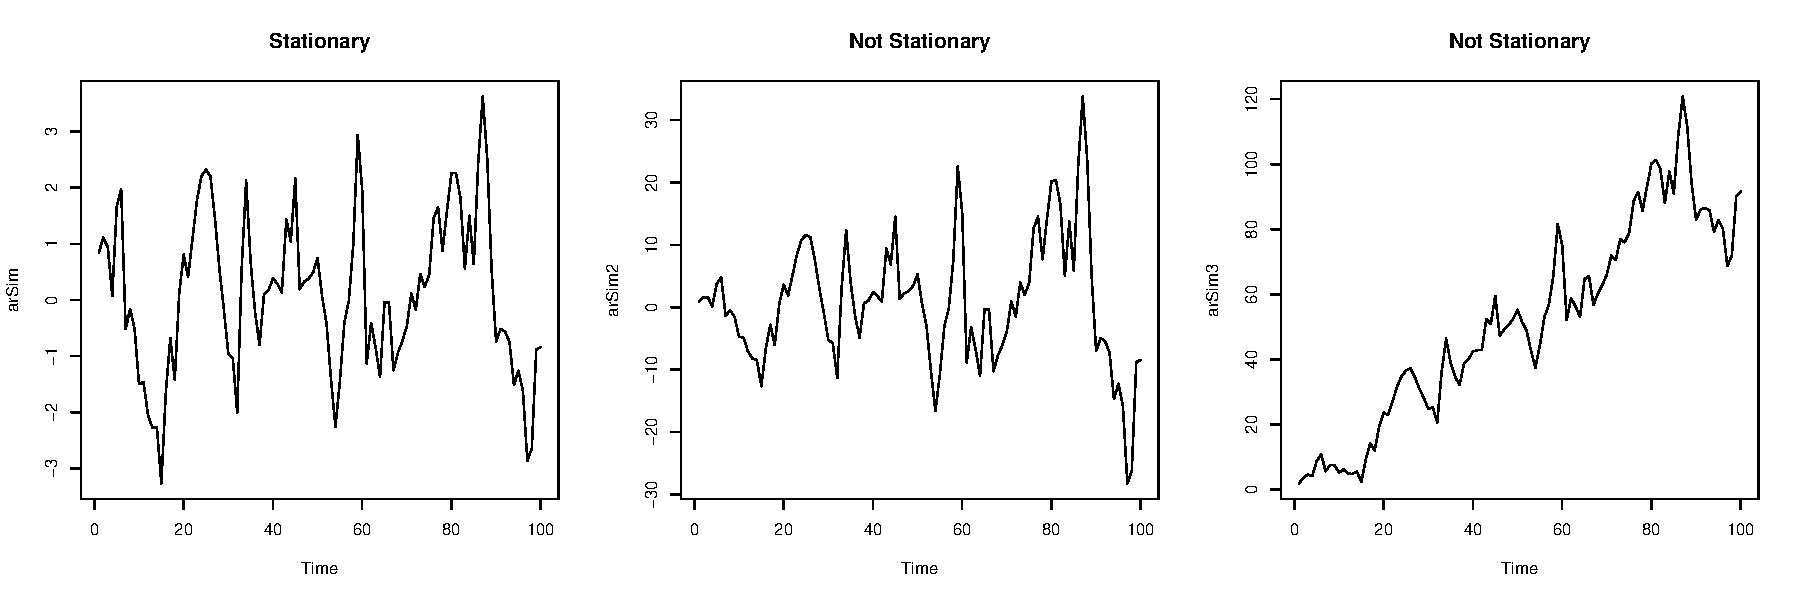
\includegraphics[width=\textwidth]{../figures/module6/tsExamples.pdf}
\caption{Examples of stationary and non-stationary time series.}
\label{fig:tsExamples}
\end{figure}

\item SAC (sample autocorrelation; ACF) plot - coming up, a useful diagnostic for stationarity
\end{itemize}

\item Remedial Measures for Non-Stationarity
\begin{itemize}
\item Non constant variance $\rightarrow$ transform $Y_t$

\item Non-constant mean: ``de-trend'' the data using a predictive model where time is the explanatory variable. 

\begin{itemize}
\item Use a scatter-plot of time vs residuals to determine an appropriate model (see Figure \ref{fig:tsExamples2}).
% Write theoretical models (using time as the sole predictor) for each case
% Sin equation $\hat{Y} = \beta_0 + \beta_1\sin(2t\pi/L) (with L being the period)
\begin{figure}
\centering
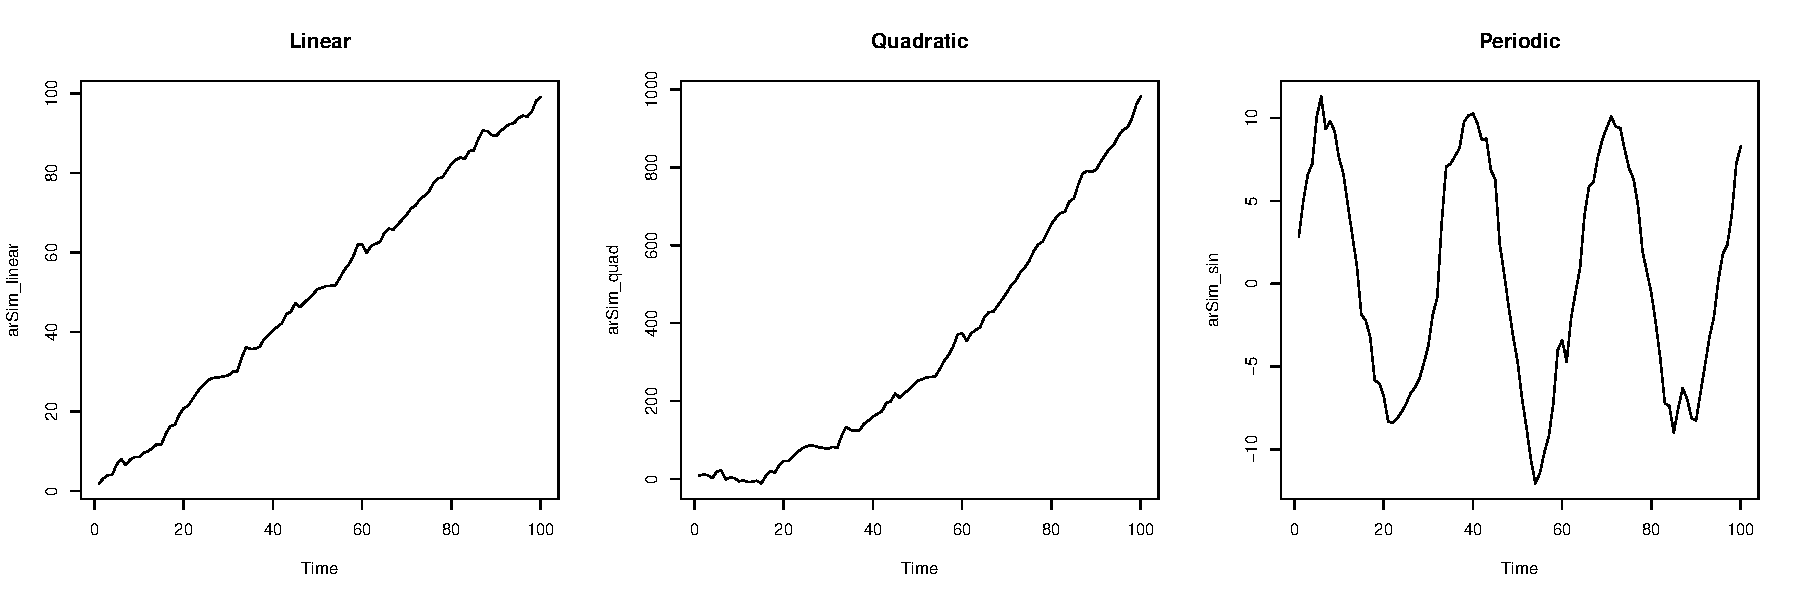
\includegraphics[width=\textwidth]{../figures/module6/tsExamples2.pdf}
\caption{Examples of different trends that may occur in a time series.}
\label{fig:tsExamples2}
\end{figure}
\end{itemize}
\item ``Differencing'' for stubborn trends:
\begin{itemize}
\item First differences: $Z_t = Y_t - Y_{t-1}, \quad (t = 2, \ldots, n)$
\item Second differences: $W_t = Z_t - Z_{t-1} = Y_t - 2Y_{t-1} + Y_{t-2} \quad (t = 3, \ldots n)$
\end{itemize}
\item HOWEVER, differencing will make periodic cycles unrecoverable, which can hurt our ability to make forecasts. 
\item For this reason, differencing is a remedial measure of last resort. 
\end{itemize}
\end{itemize}

% Second step
\item \textbf{Test for independence}

There is a difference in a series being a function of time (plus random noise) versus a series that is \textit{correlated} in time. 

%%% Question
\question{Failing to remove time-dependent trends in our data ruins our ability to check for time-dependent correlations, why is this?} 


%% Added note.
\begin{minipage}[l][2cm][c]{\textwidth}
%\begin{comment}
\note{
Points will vary together above and below the overall-average, making them look correlated, when they are actually varying randomly about the trend. 
}
%\end{comment}
\end{minipage}

AFTER removing trends, determine if the data are just ``white noise'' (no dependence structure)
$H_0:$ Data are just white noise

in SAS: $\chi^2$ test for lags 1 through $k$, (where $k$ is selected by the user). 



\item \textbf{Identify tentative dependence structures}
\begin{itemize}

 \item Notation: $Z_t$ is the \underline{stationary} time series after ``transforming''
  (including estimating out time trends and other covariates)
  the original time series $Y_1,\ldots,Y_n$\\

 \item Sample autocorrelation function (ACF or \underline{S}ACF)
    \begin{eqnarray}
      r_m & = & \mbox{linear association (correlation) between time series observations} \nonumber \\
         &   & \mbox{separated by a lag of $m$ time units} \nonumber
   \end{eqnarray}


\item \underline{PLOT 1: sample autocorrelation plot (or SAC / ACF)}: check for stationarity and identify tentative dependence structure
\begin{itemize}
  \item bar-plot $r_m$ vs. $m$ for various lags $m$
  \item lines often added to represent 2 SE's (rough significance threshold)
  \item SAC / ACF terminology:
    \begin{itemize}
      \item ``spike'' : $r_m$ is ``significant''
      \item ``cuts off'' : no ``significant'' spikes after $r_m$
      \item ``dies down'' : decreases in ``steady fashion''
    \end{itemize}



\item If $Z_t$ stationary, SAC either cuts off fairly quickly or dies down fairly quickly (sometimes in ``damped exponential'' fashion) \\ \vspace{1em}
\item If SAC dies down extremely slowly, $Z_t$ nonstationary (see Figure \ref{fig:nsACF}) \\ \vspace{1em}
%   \item Ch. 9 of Bowerman \& O'Connell: ``... if the SAC cuts off fairly quickly, it will often [but not always] do so after a lag k that is less than or equal to 2.''

\begin{figure}
\centering
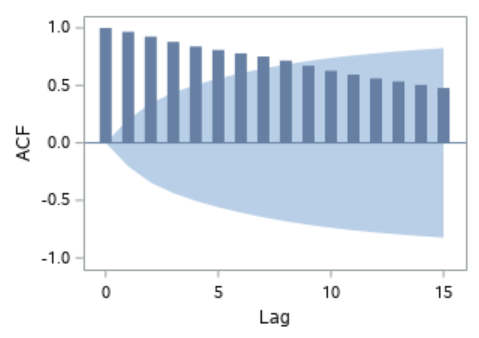
\includegraphics[width=0.6\textwidth]{../figures/module6/nsACF.png}
\caption{Sample ACF plot for a non-stationary time series.}
\label{fig:nsACF}
\end{figure}


\end{itemize}
%\end{enumerate}

\vspace{1em}

\item Sample partial autocorrelation function (PACF or \underline{S}PACF)
\begin{eqnarray}
  r_{m,m} & = & \mbox{autocorrelation of time series observations separated by a lag of $m$} \nonumber \\
  & &  \mbox{\underline{with the effects of the intervening observations eliminated}} \nonumber
\end{eqnarray}

\vspace{1em}

\item \underline{PLOT 2: sample partial autocorrelation plot (or SPAC / PACF)}
\begin{itemize}
  \item bar-plot $r_{m,m}$ vs. $m$ for various lags $m$
  \item lines often added to represent 2 SE's (rough significance threshold)\\
\end{itemize}


\item Main dependence structures

\begin{enumerate}

\item \underline{AR(p) dependence structure}: autoregressive process of order $p$:
\begin{itemize}
\item current time series value depends on past values; common representation for AR(p):
\begin{eqnarray}
Z_t & = & \delta + \phi_1 Z_{t-1} + \phi_2 Z_{t-2} + \ldots + \phi_p Z_{t-p} + a_t \nonumber
\end{eqnarray}
    \begin{itemize}
      \item $\phi_i$ are unknown parameters; random shock $a_t$ iid $N(0,\sigma^2)$
    \end{itemize}
\item identify using SPAC:
  first $p$ terms of SPAC will be non-zero, then drop to zero (sketch)\\ \vspace{3em}
\end{itemize}


\item \underline{MA(q) dependence structure}: moving average process of order $q$:
 \begin{itemize}
    \item current time series value depends on previous random shocks
    \item model:\\ \vspace{-2em}
\begin{eqnarray}
  Z_t & = & \delta + a_t - \theta_1 a_{t-1} - \theta_2 a_{t-2} - \ldots - \theta_q a_{t-q} \nonumber
\end{eqnarray}
\begin{tabular}{l l l}
   $Z_t$ : stationary ``transformed'' time series  & &  $\theta_i$ : unknown parameters\\
   $a_t$ : random shocks  & & $\delta$ : unknown parameter
\end{tabular}

  \vspace{1em}

   \item identify using SAC:
  first $q$ terms of SAC will be non-zero, then drop to zero (sketch)\\ \vspace{4em}
\end{itemize}

\end{enumerate}

\end{itemize}

\vspace{1em}


\begin{tabular}{c l l}
\multicolumn{3}{c}{\underline{Common Dependence Structures for Stationary Time Series}} \\
& & \\
  & SAC & SPAC \\ \hline
 & \\
MA(1) & cuts off after lag 1 & dies down, dominated by\\
  & & damped exponential decay \\
 & \\
MA(2) & cuts off after lag 2 & dies down, in mixture of\\
  & & damped exp. decay \& sine waves \\
 & \\
AR(1) & dies down in damped & cuts off after lag 1\\
  & exponential decay & \\
 & \\
AR(2) & dies down, in mixture of & cuts off after lag 2\\
 & damped exp. decay \& sine waves & \\
 & \\
ARMA(1,1) & dies down in damped exp. decay & dies down in damped exp. decay\\
 & \\ \hline
\end{tabular}

\vspace{3em}

\underline{ARIMA(p,d,q) dependence structure}:  Autoregressive {\bf Integrated}  Moving Average Model
\begin{itemize}
  \item a \underline{very} flexible family of models  $\Rightarrow$ useful prediction
  \item recall first difference: $Z_t = Y_t - Y_{t-1}$, $t=2,\ldots,n$\\
        and second difference: $W_t  = Z_t - Z_{t-1} = Y_t - 2 Y_{t-1} + Y_{t-2}, \mbox{}t=3,\ldots,n$
  \item after differencing, AR and MA dependence structures may exist: ARIMA(p, {\bf d} ,q)
    \begin{itemize}
      \item p : AR(p) -- value at time $t$ depends on previous $p$ values)
      \item d : \# of differences (need to take $d^{th}$ difference to make stationary)
      \item q : MA(q) -- value at time $t$ depends on previous $q$ random shocks)
    \end{itemize}
  \item use SAC and SPAC to select $p$ and $q$ -- but how to select $d$?
    \begin{itemize}
      \item usually look at plots of time series
      \item choose lowest $d$ to make stationary (also SAC)
    \end{itemize}
  \item sometimes see backshift notation:  $B Y_t = Y_{t-1}$
    \begin{itemize}
      \item $d=1$ : $Z_t = Y_t - Y_{t-1} = Y_t - B Y_t = (1-B) Y_t$
      \item general $d$: $Z_t = (1-B)^d Y_t$\\
    \end{itemize}

  \item ``Fit model'' $\rightarrow$ estimates \& standard errors for $\beta_j$'s, $\phi_l$'s, \& $\theta_l$'s\\

  \item Several approaches exist to estimate $\phi_l$'s, $\theta_l$'s, and $\beta_j$'s, and  deal with initial lag; we'll use
ULS (unconditional least squares) for MA(q) \& AR(p)\\



\item ARIMA(p,d,q) model rewritten, with $t=1,\ldots,n$:
\begin{eqnarray}
Y_t & = & g_1(Y_1,\ldots,Y_{t-1}) + g_2(X_{t,1},\ldots,X_{t,k-1}) + g_3(a_1,\ldots,a_t) \nonumber \\
 & & \mbox{\hspace{-3em} where}\nonumber \\
 g_1 & = & \mbox{linear combination (LC) of previous observations} \nonumber \\
 %& & \mbox{(Differencing)} \nonumber \\
 g_2 & = & \mbox{LC of predictors at time $t$, in terms of parameters $\beta_j$} \nonumber \\
 % & & \mbox{(Linear Model)} \nonumber \\
 g_3 & = & \mbox{function of random shocks in terms of parameters $\phi_l$ \& $\theta_l$} \nonumber
 %& & \mbox{(AR \& MA dependence structures)} \nonumber
\end{eqnarray}

%% Added note.
\begin{minipage}[l][2cm][c]{\textwidth}
%\begin{comment}
{\color{red}
\begin{tabular}{ll}
$g_1$ & differencing \\
$g_2$ & linear model with predictors
$$
\end{tabular}
}
%\end{comment}
\end{minipage}

\end{itemize}

\vspace{1em}

\item \textbf{Fit dependence structures and assess model adequacy}
\begin{itemize}


\item General SAS code for ARIMA(\underline{p},\underline{d},\underline{q}), $Y$ in terms of $X_1,\ldots,X_{k-1}$:\\

\vspace{-.5em}

\verb7 proc arima data = a1;7\\
\verb7  identify var = 7\underline{$Y$} \verb7(7\underline{$d$} \verb7)  crosscorr = (7\underline{$X_1 \ldots X_{k-1}$}\verb7) ;7\\
\verb7  estimate p = 7\underline{$p$}\verb7  q = 7\underline{$q$}\verb7  input = (7\underline{$X_1 \ldots X_{k-1}$}\verb7)  method = uls  plot;7\\
\verb7  forecast lead = 7\underline{$L$}\verb7 alpha = 7\underline{$a$}\verb7 noprint out = fout;7\\
\verb7 run;7

\begin{tabular}{l l l}
\hspace{4em} & option & description \\ \cline{2-3}
& \underline{d}, \underline{p}, \underline{q} & differencing, AR, \& MA settings (as before) \\
& \verb7plot7 & adds RSAC \& RSPAC plots \\
& \underline{L} & \# times after last observed to forecast \\
& \underline{a} & set confidence limit; \underline{a} = .10 $\Rightarrow$ 90\% conf. limits \\
& \verb7noprint7 & optional, suppresses output \\
& \verb7out = fout7 & optional, sends forecast data to \verb7fout7 data set\\
\end{tabular}


\item Useful diagnostics for ``goodness of fit'':
\begin{itemize}
  \item{Numerical}
    \begin{itemize}
       \item Standard Error -- measure of ``overall fit''; in SAS: \verb7Std Error Estimate7
           \begin{eqnarray}
             S & = & \sqrt{\frac{ \sum_1^n (Y_t - \hat{Y}_t)^2}{n-n_p} } \mbox{, \hspace{1em} $n_p$ = \# parameters in model} \nonumber
            \end{eqnarray}
             
\begin{minipage}[l][1cm][c]{\textwidth}
%\begin{comment}
{\color{red}
Note that $S$ is similar to $\sqrt{\text{MSE}}$
}
%\end{comment}
\end{minipage}
            
       \item Ljung-Box statistic $Q^*$ (\& p-value);\\
       in SAS: lag 6 $\chi^2$ for \verb7Autocorrelation Check of Residuals7
          \begin{itemize}
             \item basic idea: look at ``local'' dependence among residuals in first few sample autocorrelations
             \item under $H_0$: ``model is adequate'', $Q^* \sim \chi^2_{df}$
          \end{itemize}
    \end{itemize}

  \item Graphical (\underline{PLOTS 3 and 4}) -- focus on residuals% (after accounting for dependence structure)
    \begin{itemize}
        \item Residual sample autocorrelation plot (RSAC)
        \item Residual sample partial autocorrelation plot (RSPAC)
    \end{itemize}
\end{itemize}

\end{itemize}

        
%%% Question
\question{How will we know from these plots if we ``succeeded''?}


%% Added note.
\begin{minipage}[l][3cm][c]{\textwidth}
%\begin{comment}
{\color{red}
We should see no significant autocorrelations, which would suggest that we have fully accounted for the time dependent structure in the data. 

\vspace{1em}
ANALOGY: Mining - we are trying to extract information from data, and unaccounted structure is like knowing we left gold in the ground. 
}
%\end{comment}
\end{minipage}


\vspace{1em}

\item \textbf{Using adequate model:}
    \begin{enumerate}
     \item forecast response (*** w/ conf. interval ***) -- careful far beyond data
     % (note conf interval flare-out)
     \item test model terms (incl. predictor variables, but also AR \& MA parameters)
    \end{enumerate}


\end{enumerate}

\end{document}